\chapter{Concept}
\section{Tree Creation}
\label{sec:tree_creation_angle}
In \acrshort{acr:CPlan} genetic optimisation algorithms based on trees as chromosomes were already implemented. They had no solution to produce trees from existing graphs. The newly created tree generation algorithm produces a relative tree with absolute angles. This allowed an easier and faster work process with tree based structures.

To create a tree from an existing graph the angle and distance should be enough data to fully represent a graph.
Two approaches exist to define angles. One is to separate the circle range into minus and plus 180 degrees. This would allow to step straight forward with the angle 0 degree (Figure \ref{fig:tree-generation-decision} left). Another approach is to use the range from 0 to 360 degrees. In this case straight forward would be 180 degrees (Figure \ref{fig:tree-generation-decision} right).

\begin{figure}[!ht]
    \centering
    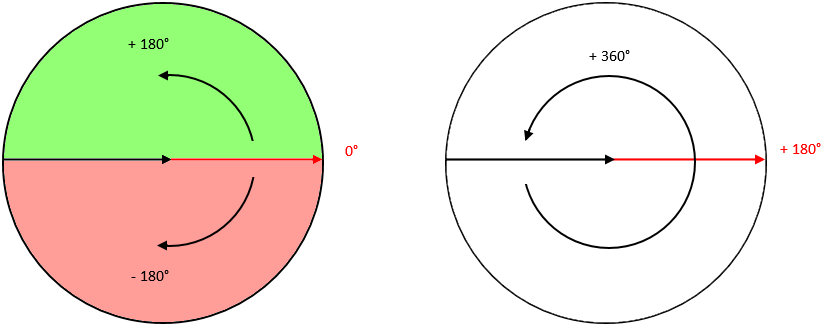
\includegraphics[width=\textwidth]{tree-generation-decision.png}
    \caption{Degree separation method \label{fig:tree-generation-decision}}
\end{figure}

Because a tree can not fully represent a graph, many points exist multiple times in the resulting tree. During recreation of a graph this should be considered.

\FloatBarrier
\pagebreak
\section{K-Means}
Clustering is an approach to group input data. These groups are called clusters. To separate a street network in CPlan into reasonable parts this approach could be used. As described in section \ref{sec:K-Means}, the K-Means algorithm assigns data points to different clusters by using the minimal distances to centroids. For this thesis the position feature (x and y coordinates of the road junctions) are used.

The used features ignore the graph structure of the street network. As a result clusters are not always connected subgraphs. This means it could lead to unexpected transitions between clusters.

\subsection{Connected Cluster Approach} \label{sec:connected_cluster_approach}
To solve the problem of unexpected transitions between clusters the best result of the K-Means algorithm tries can be combined with the distance measurement of a \acrlong{APSP} (\acrshort{APSP}) algorithm (Dijkstra / Floyd-Warshall) to assign the edges to a cluster. These algorithms are described in more detail in the background chapter \ref{sec:shortest_path}.

\subsection{Additional Features}
Different measurement methods were implemented to rate a created cluster (section \ref{sec:cluster_analysis_impl}). These features described in section \ref{sec:clusterRating} like the block size or the median street length could be used to cluster the street networks.

\pagebreak
\section{Hierarchical Clustering}
Hierarchical clustering is another area of clustering algorithms. As already mentioned in the background chapter \ref{sec:hierarchicalClustering} this clustering algorithm can use other distances than the euclidean distance. This advantage was utilised to cluster the street network with the shortest path between vertices in the graph as a distance instead of using the positions (x and y coordinates) as features. This method is referred to as graph distance in this document.

The improvement of utilizing graph distances over the usage of euclidean distances when applying hierarchical clustering is that the resulting clusters will always be connected subgraphs. Furthermore, the hierarchy that results from this clustering approach can be used to create any number of clusters from $1$ to $n$, where $n$ is the number of vertices.

The following approach provided itself as reasonable to create the described clustering:

\begin{enumerate}
    \item Compute \acrshort{APSP} algorithm for the given street network graph
    \item Generate hierarchy by running hierarchical clustering with chosen reduction formula (This uses the distances calculated in step 1)
    \item Create wished number of clusters from this resulting hierarchy
\end{enumerate}

\subsection{Distance caching} \label{sec:concept_distance_caching}
To reach an appropriate time complexity when computing hierarchical clustering using \acrshort{UPGMA} or \acrshort{WPGMA} reduction formulae, distances between clusters have to be cached. If those distances were calculated every time --- by iterating over all nodes contained by two clusters --- it would inflict bad performance. The speedup of this improvement is further discussed in section \ref{sec:measurements-speed}.

\subsection{Hight Memory Usage} \label{sec:concept_memory_usage}
The most trivial solution to store those discussed distances (\acrshort{APSP} and cached cluster distances) would be as a matrix of double-precision floating-point numbers. It is the most trivial solution because the positions were already stored in this number format and matrix data structures are easily accessible. The \acrshort{APSP} and cached distances can be stored in the same matrix, because when using agglomerative hierarchical clustering, each vertex is also one of the initial clusters.

This storage strategy would use $(2n-1)^2$ double-precision floating-point numbers, $n$ being the node count (number of junctions). As an example: For the used environment this storage strategy would amount to about 21.7 Gigabyte of used memory for the street network of Zurich. In section \ref{sec:memory_usage} of the implementation chapter three implemented optimisations are described.

\subsection{Clusters of Highly Varying Sizes} \label{sec:concept_cluster_sizes}
Hierarchical clustering can sometimes result in clusters with high differences of the vertex count. In figure \ref{fig:problem_unmodified_cluster_size} a clustering of Weimar with such a case is shown. In this figure there is a relatively big cluster in the centre of the city and at the bottom left corner are multiple very small clusters.

Depending on the desired further use of the clusters, more equally sized clusters are favoured. Section \ref{sec:outout_modification} describes, how these modified cluster sizes were achieved.

\begin{figure}
    \centering
    \begin{mdframed}[style=mdthight, userdefinedwidth=0.5\linewidth, align=center]
        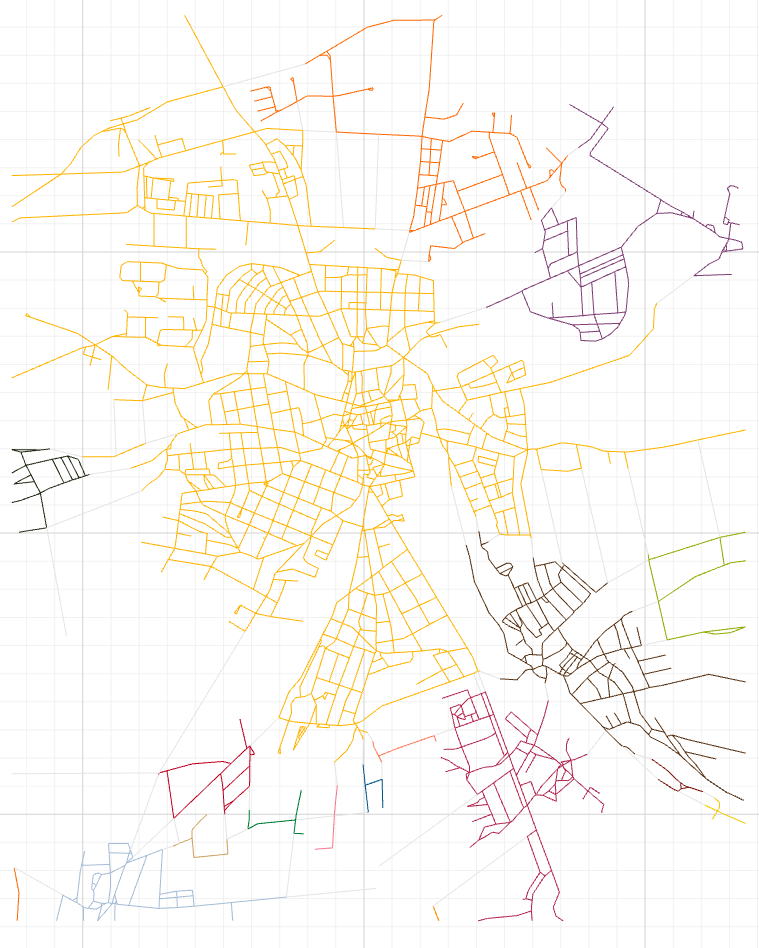
\includegraphics[width=\linewidth]{unmodified_cluster_size.png}
    \end{mdframed}
    \caption{Clustering with highly varying cluster sizes}
    \label{fig:problem_unmodified_cluster_size}
\end{figure}

\pagebreak
\section{Cluster Analysis}
\label{sec:concept_cluster_analysis}
To measure and compare the different areas they should be characterized. Therefore some districts with noticeable characteristics haven been selected and compared to each other. The found characteristics could help to separate a given city on a feature based approach.
These areas have been selected with the aide of Jun.-Prof Dr Reinhard König from the ETH Zurich.

\subsection{Historic District}
\label{sec:historyDistinct}
This district is characterised by a high count of short streets with many connections. As a result the block areas are small and the block count per area is high. Additionally the mean angles are high and the density (convex hull area divided by total street length) is low. This characteristics can be observed in the image \ref{fig:historic_district}.

\begin{figure}[!ht]
    \centering
    \begin{mdframed}[style=mdthight, userdefinedwidth=0.4\textwidth, align=center]
        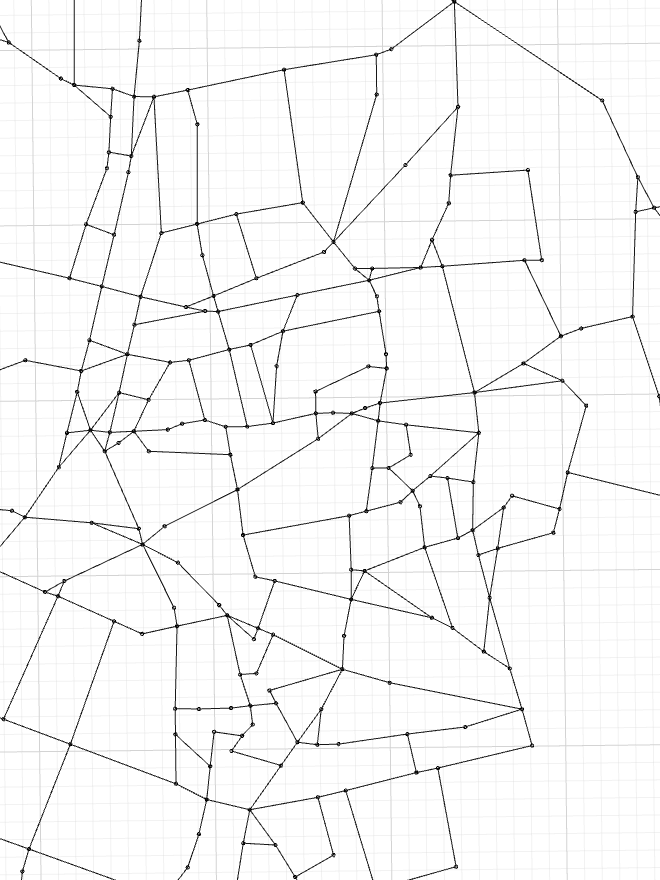
\includegraphics[width=\linewidth]{district_historic.png}
    \end{mdframed}
    \caption{Historic District of Weimar}
    \label{fig:historic_district}
\end{figure}

\FloatBarrier
\subsection{Business / Manhattan District} 
\label{sec:businessDistinct}
If the relative block area (block area divided by surrounding circle area) is high the given subgraph is probably a business/Manhattan district. The mean connection count and the density compared with a historic district (section \ref{sec:historyDistinct}) should be much higher. An example business district can be found on the map of Weimar (figure \ref{fig:business_district}).

\begin{figure}[!ht]
    \centering
    \begin{mdframed}[style=mdthight, userdefinedwidth=0.4\textwidth, align=center]
        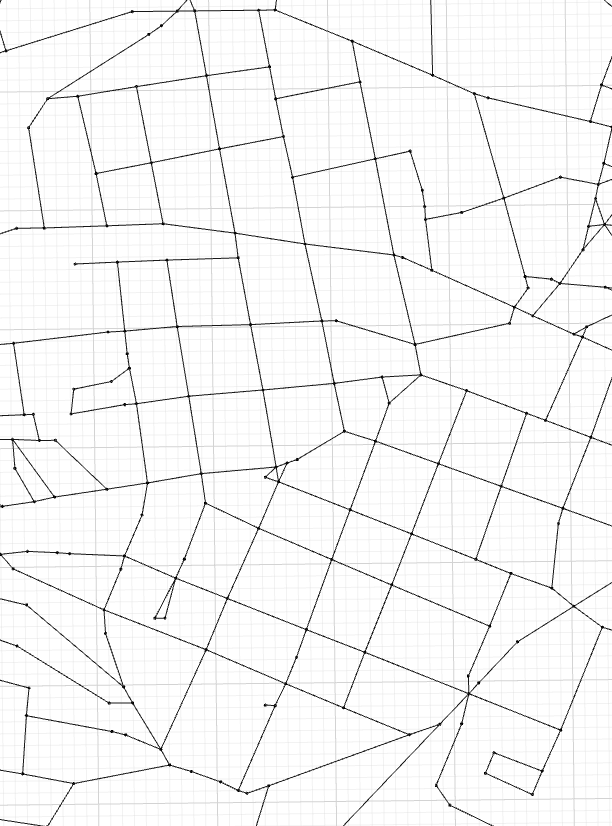
\includegraphics[width=\linewidth]{district_business.png}
    \end{mdframed}
    \caption{Business District of Weimar}
    \label{fig:business_district}
\end{figure}

\FloatBarrier
\subsection{Outskirts Area}
\label{sec:outskits}
These areas are characterized by extreme long streets and a low connection count. As a result the density is very high. The block count is compared with a business or historic district exceptionally low. In figure \ref{fig:outskirts_district} these characteristics can be found.

\begin{figure}[!ht]
    \centering
    \begin{mdframed}[style=mdthight, userdefinedwidth=0.6\textwidth, align=center]
        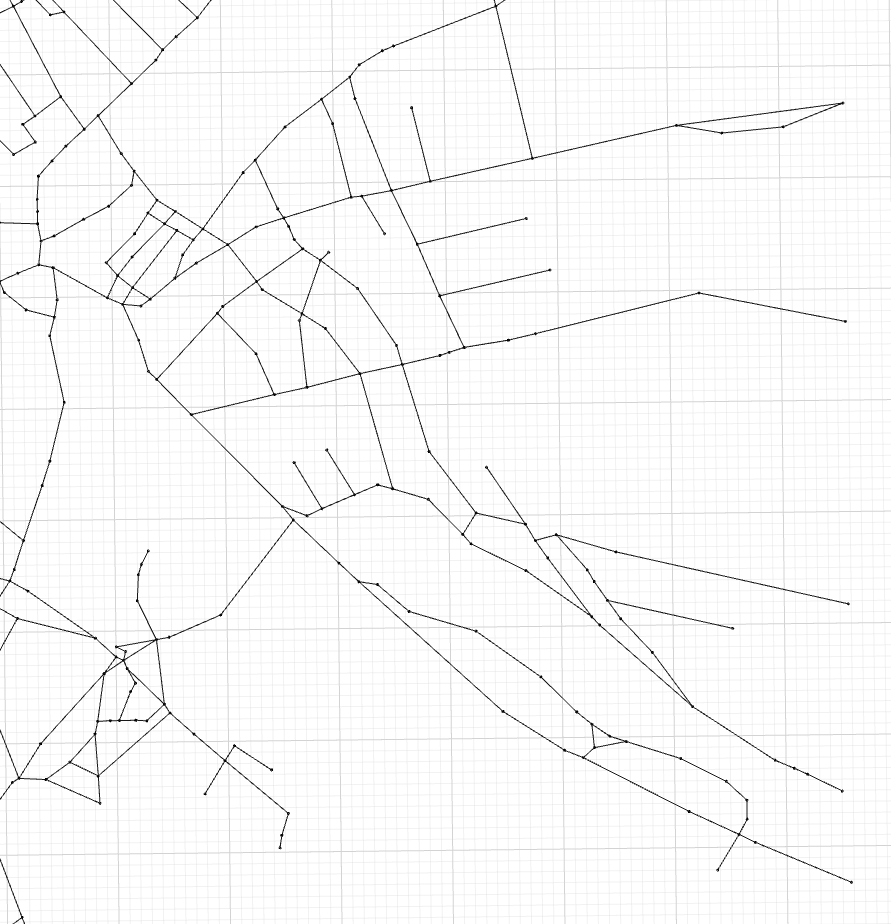
\includegraphics[width=\linewidth]{district_outskirts.png}
    \end{mdframed}
    \caption{Outskirts Area of Weimar}
    \label{fig:outskirts_district}
\end{figure}